\documentclass[]{report}
\usepackage[]{tgpagella}
\usepackage{amsmath}
\usepackage{parskip}
\usepackage{matlab-prettifier}
\usepackage[]{circuitikz}
\usepackage[]{xcolor}
\usepackage[]{listings}
\usepackage{graphicx}
\usepackage{float}
\usepackage{booktabs}
\usepackage[left=2.5cm, right=2.5cm, bottom=2.5cm]{geometry}



\definecolor{smoky}{gray}{0.85}

\title{\textbf{ECE/MEDBIO 4455} \\ Biomedical Systems Analysis \\ \textit{MATLAB Investigation 1}}
\author{Arnav Goyal  \\ Helen Zhou  \\ Yucong Wang }


\begin{document}

\maketitle
\newpage
\tableofcontents
\newpage

%% QUESTION 1
\chapter*{Questions, Answers, \& Explanations}
\addcontentsline{toc}{chapter}{Questions, Answers, \& Explanations}  % add to ToC

\section*{Question 1a}
\addcontentsline{toc}{section}{Question 1a}  % add to ToC

Based on the tilts, phase durations, and load resistance reported for the \textbf{fixed-tilt} waveform in $\tau_g$, and the source 
capacitor, $C_g$.


The values attained from the fixed-tilt waveform from \textit{Hayashi et al.} are noted below

\begin{itemize}
 	\item $\text{tilt}_{d1}  = 0.65$ 
 	\item $\text{tilt}_{d2}  = 0.65$
	\item $t_{d1} = 10$ ms
	\item $t_{d2} = 10$ ms
	\item $E        = 40$ J
	\item $R_\text{meas}   = 84 \ \Omega$
\end{itemize}
 
One can estimate the stimulus time-constant $\tau_g$, through equation \ref{eq:1} only by knowing the phase duration and the tilt value. Note that this equation is only applicaple to a monophasic decaying exponential. For the case of the biphasic decaying exponential, we can split it up into its two phases.

\textit{Note:} Doing this results in the same value for both phases, as the tilt and duration are the same values across both phases of the biphasic decaying exponential

\begin{equation}
\label{eq:1}
	\text{Tilt} = 1 - \exp{\left( - \frac{t_d}{\tau_g} \right)}
\end{equation}

Rearranging to solve for $\tau_g$ we obtain  the following value after using the values from \textit{Hayashi et al.}

\[
	\tau_g = - \frac{t_d}{\ln{\left( 1 - \text{Tilt} \right)}} = 9.5254 \text{ ms}	
\]

Once we have the value of $\tau_g$, we can use the commonly known RC time-constant equation to solve for $C_g$.

\begin{equation}
\label{eq:2}
	\tau = R \cdot C
\end{equation}

In our case we would use the resistance of $R_\text{meas}$, and the time constant value $\tau_g$ we solved for earlier. Solving equation \ref{eq:2} gives the following value for $C_g$

\[
	C_g = \frac{\tau_g}{R_\text{meas}} = 113.397 \,\mu\text{F}
\]

Since this is intended to be a MATLAB investigation, we can numerically solve this with the MATLAB code below.

\begin{lstlisting}[style=Matlab-editor, backgroundcolor=\color{smoky}]
%% use params from fixed tilt waveform (defib unsuccessful)
tilt_d1  = 0.65; % pc
tilt_d2  = 0.65; % pc
phase_d1 = 10  ; % ms
phase_d2 = 10  ; % ms
E        = 40  ; % J
R_meas   = 84  ; % ohm

%% Solve for capacitor tau_g value with the above values
tau_g = - 0.010 / log(1 - tilt_d1) % s

%% now with tau_g solve C_g
C_g = tau_g / R_meas % F
\end{lstlisting}

\section*{Question 1b}
\addcontentsline{toc}{section}{Question 1b}  % add to ToC

Is the value you obtained for $C_g$ realistic? Cite evidence to support your response. 

Yes, our value for $C_g$ is realistic [1] shows values for $C_g$ in the same range (106-177) $\mu$ F. Our value for  from $C_g$ falls nicely within this range.

[1] M. Kroll and C. Swerdlow, “Optimizing defibrillation waveforms for ICDS,” Journal of Interventional Cardiac Electrophysiology, vol. 18, no. 3, pp. 247–263, Jun. 2007. doi:10.1007/s10840-007-9095-z 

\section*{Question 2a}
\addcontentsline{toc}{section}{Question 2a}  % add to ToC

Using your results from Question 1 and the phase durations reported for the \textbf{tuned-duration 
waveform} in the \textit{Hayashi et al.} case study, reverse engineer the DeFT Response algorithm the 
authors employed to tune the waveform by completing for following steps. State separate criteria to determine an optimal first-phase duration, $t_{d1}$, and an optimal second
phase duration, $t_{d2}$.

\textbf{Optimal td1:} should be equal to the time required for the transmembrane voltage (Vm) to reach its peak value;

\textbf{Optimal td2:} should be just long enough to return the transmembrane voltage from its peak back to the resting potential without causing significant hyperpolarization.


\section*{Question 2b}
\addcontentsline{toc}{section}{Question 2b}  % add to ToC

Observe from the input arguments for \texttt{ biphasic\_exp\_tuned\_dur.m } that the only parameter 
we do not yet have a value for that is needed to compute the heart’s voltage response, Vm(t), is $\tau_m$.\\ 
Use \texttt{ biphasic\_exp\_tuned\_dur.m } to search for values of $\tau_m$ that yields same optimal durations as reported in paper. Report your $\tau_m$ values to 0.1 ms precision. (You should obtain different $\tau_m$ values from the optimization criteria for $t_{d1}$ and $t_{d2}$)

From question 2a  we know the separate criterion for optimal phase 1 and 2 durations are:
\begin{itemize}
	\item An optimal $t_{d1}$ is just long enough for the membrane voltage to peak
	\item An optimal $t_{d2}$ is just long enough for the membrane voltage to go back down to 0V
\end{itemize}

We can write a MATLAB script that performs a linear search over a range  for $tau_m$. It can run the provided \texttt{biphasic\_exp\_tuned\_dur.m} function to compute the membrane-voltage response $V_m(t)$.

We can use this response to find two things. First, a $\tau_m$ optimized according to phase 1 where the membrane voltage peaks at the reported optimal time. Second, another $\tau_m$ optimized according to phase 2 where the membrane voltage returns back to 0V after the reported optimal time.

Before we write a MATLAB script, we should consider how we would approach this problem without the use of MATLAB, this will help to develop the proper algorithm. We will also note that since we are computing the tuned duration response, we need to use the \textbf{tuned-duration} numbers reported by \textit{Hayashi et al.} for this question, these numbers are listed below

\begin{itemize}
	\item $t_{d1} = 4.5$ ms
	\item $t_{d2} = 2.0$ ms
	\item $E = 28.4$ J
\end{itemize}

so what we need to do in MATLAB is try to solve the below equation for $\tau_m$ Ths should give us our first $\tau_m$ value.

\[
V'_m(t_{d1}) = 0
\]


\textit{Note:} Because we are doing this with floating-point values in MATLAB the derivative will rarely be zero, so we will assume the peak occurs when the derivative is at the minimum value.

The MATLAB script that finds the optimal phase 1 $\tau_m$ to 0.1 ms precision is given below. \newpage

\begin{lstlisting}[style=Matlab-editor, backgroundcolor=\color{smoky}, basicstyle=\ttfamily\tiny]
clear all;

%% load in previously found C-g tau-g
C_g   = 113.397; % uF
tau_g = 9.5254;  % ms

%% load in tuned duration paper numbers
R_meas = 84;   % Ohm
t_d1   = 4.5;  % ms
t_d2   = 2.0;  % ms
E      = 28.4; % J


%% define a search range for tau_m values for optimal t-d1
tau_m_guesses = 2.3:0.0001:2.6;
root_times    = zeros(length(tau_m_guesses));

for i = 1:length(tau_m_guesses)
	% get membrane voltage response
	[Vg, Vm, t] = biphasic_exp_tuned_dur(tau_m_guesses(i), C_g, E, R_meas, t_d1, t_d2, 'n');
	
	% take ddt and find where its at its minimum
	% due to FP values it will never be exactly 0 so we have to consider the minimum here
	dVm  = diff(Vm);
	root = find( abs(dVm) == min(abs(dVm)), 1 );
	
	%% with the root index we can find the time (ms) of the zero
	precision = 1e-5; % the provided function has us time-precision
	root_time = root * precision;
	root_time = 1e3 * root_time; % convert to ms
	
	% print info
	fprintf('Iteration: %d | Current tau_m: %f | Root Time: %f ms\n', i, tau_m_guesses(i), root_time)
	
	% store the root time
	root_times(i) = root_time;
end

% now find the root-time closest to t_d1 and grab the corresponding tau_m_guess

best_tau_m_index = find( abs(root_times - t_d1) == min(abs(root_times - t_d1)), 1 );
fprintf('Best tau-m index for optimal phase 1: %d\n', best_tau_m_index);

best_tau_m     = tau_m_guesses(best_tau_m_index);
best_root_time = root_times(best_tau_m_index);
fprintf('Best tau-m: %f, with root-time: %f\n', best_tau_m, best_root_time);

% plot the optimal tau_m graph 
[Vg, Vm, t] = biphasic_exp_tuned_dur(best_tau_m, C_g, E, R_meas, t_d1, t_d2, 'y');
\end{lstlisting}

This script iterates over several $\tau_m$ values and provides this value (along with the other determined values) to the tuned-duration function provided in the lecture material. This function will compute the stimulus and membrane voltage responses. The membrane response will be differentiated with the diff() function, and the root-time will be stored in an array. After going through all iterations for $\tau_m$ the script checks the one with the root-time closest to the desired 4.5 ms and prints this value.

This script finds that the best $\tau_m$ guess to optimize phase 1 is 2.4640 ms. A plot of this response is provided in Figure \ref{fig:phase1}.

\begin{figure}[H]
	\centering
	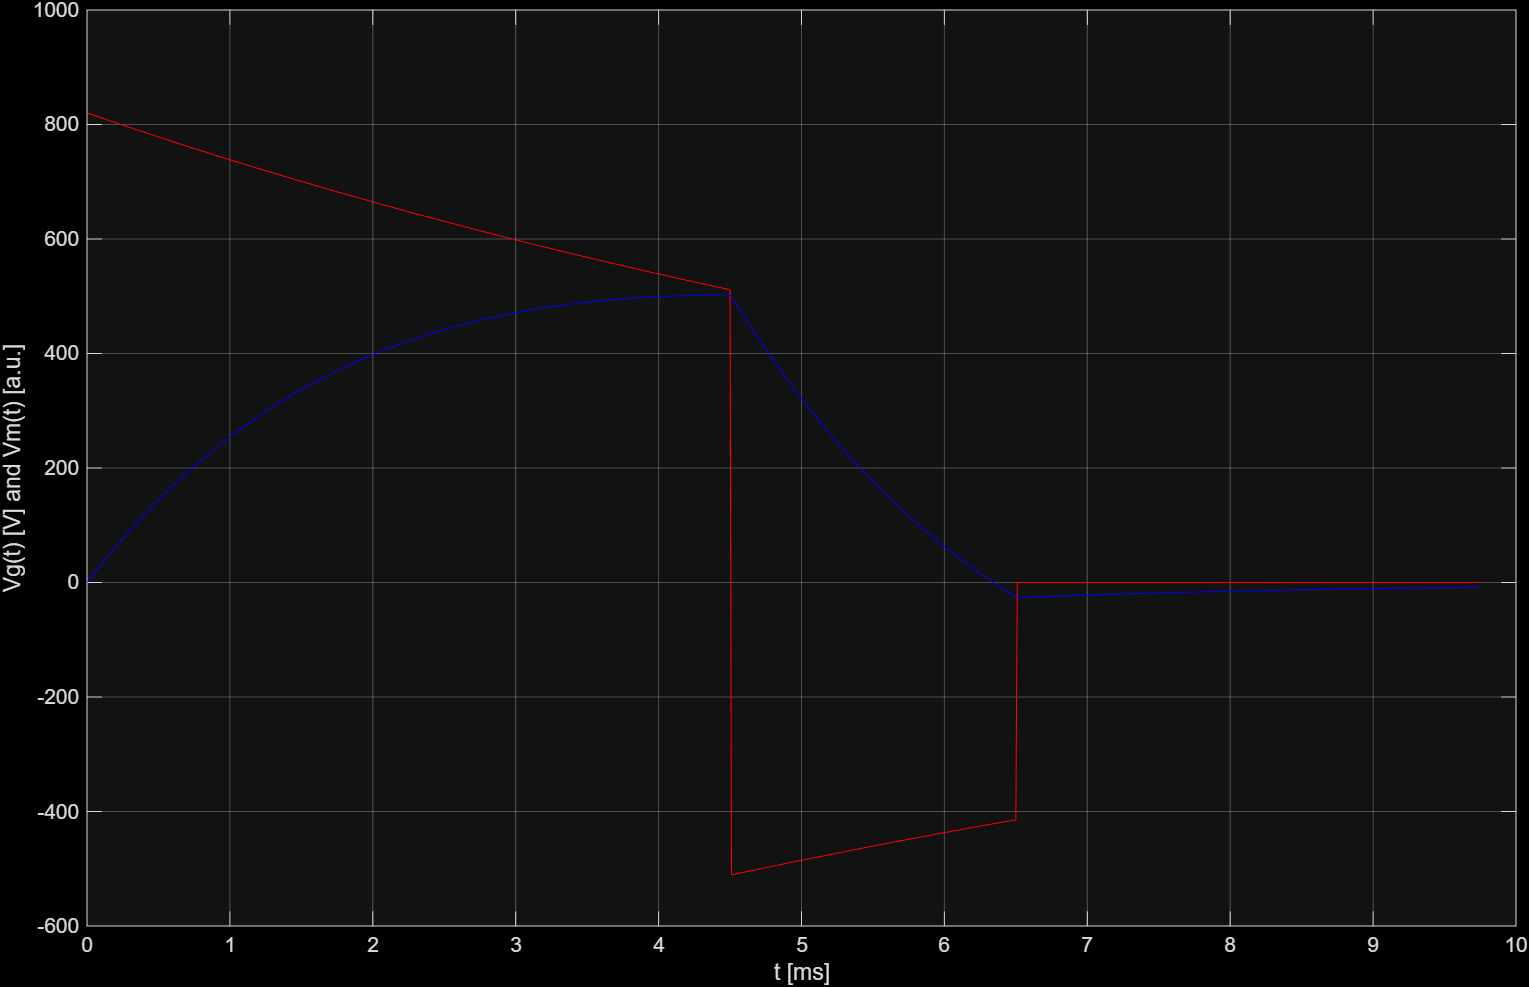
\includegraphics[width=0.7\textwidth]{phase1_response.png}
	\caption{\textcolor{red}{\textbf{Stimulus}} \& \textcolor{blue}{\textbf{Membrane}} Voltage Response over Time, Optimized for $t_{d1}$}
	\label{fig:phase1}
\end{figure}


\subsection*{Optimizing the Second-Phase}

To optimize the second phase we need to consider that the goal is to get the myocardium back to resting potential as fast as possible, without using too much energy. To do this its much more simple than phase 1, all we need to do is to ensure that the output response $V_m (t)$ goes to zero at a time $t_{d1} + t_{d2}$.

In other words, we need to solve the below for $\tau_m$ such that the below holds true.

\[
	V_m (t_{d1} + t_{d2}) = 0
\]

This is because the paper reports the \textit{phase} durations, not the total time. So the actual time at which $V_m (t)$ must go to zero can be found by adding these durations together. We can make a few modifications to our script from before in order to do this quite easily. The MATLAB code is given below

\begin{lstlisting}[style=Matlab-editor, backgroundcolor=\color{smoky}, basicstyle=\ttfamily\tiny]
clear all;

%% load in previously found C-g tau-g
C_g   = 113.397; % uF
tau_g = 9.5254;  % ms

%% load in tuned duration paper numbers
R_meas = 84;   % Ohm
t_d1   = 4.5;  % ms
t_d2   = 2.0;  % ms
E      = 28.4; % J


%% define a search range for tau_m values for optimal t-d2
tau_m_guesses = 2.3:0.0001:2.8;
root_times    = zeros(length(tau_m_guesses));

for i = 1:length(tau_m_guesses)
	% get membrane voltage response
	[Vg, Vm, t] = biphasic_exp_tuned_dur(tau_m_guesses(i), C_g, E, R_meas, t_d1, t_d2, 'n');
	
	% for optimizing td2 we need the root of Vm to be around t_d1 + t_d2 ms
	% before we find the min we must strip the start away a bit
	% this is because Vm starts at 0
	Vm = Vm(50:end);
	root = find( abs(Vm) == min(abs(Vm)), 1 );
	
	% with the root index we can find the time of the zero
	precision = 1e-5;
	root_time = root * precision;
	root_time = root_time * 1e3; % convert to ms
	
	% print info
	fprintf('Iteration: %d | Current tau_m: %f | Root Time: %f ms\n', i, tau_m_guesses(i), root_time)
	
	% store the root time
	root_times(i) = root_time;
end

% now find the root-time closest to t_d1 + t_d2 and grab the corresponding tau_m_guess

t_d = t_d1 + t_d2

best_tau_m_index = find( abs(root_times - t_d) == min(abs(root_times - t_d)), 1 );
fprintf('Best tau-m index for optimal phase 2: %d\n', best_tau_m_index);

best_tau_m     = tau_m_guesses(best_tau_m_index);
best_root_time = root_times(best_tau_m_index);
fprintf('Best tau-m: %f, with root-time: %f\n', best_tau_m, best_root_time);

% plot the optimal tau_m graph 
[Vg, Vm, t] = biphasic_exp_tuned_dur(best_tau_m, C_g, E, R_meas, t_d1, t_d2, 'y');
\end{lstlisting}

This script iterates over several $\tau_m$ values and provides this value (along with the other determined values) to the tuned-duration function provided in the lecture material. This function will compute the stimulus and membrane voltage responses. The membrane response's root-time will be stored in an array. After going through all iterations for $\tau_m$ the script checks the one with the root-time closest to the desired 6.5 ms and prints this value.

The script finds that the best $\tau_m$ value to optimize phase 2 is 2.7270 ms. A plot of this response is provided in Figure \ref{fig:phase2}.

\begin{figure}[H]
	\centering
	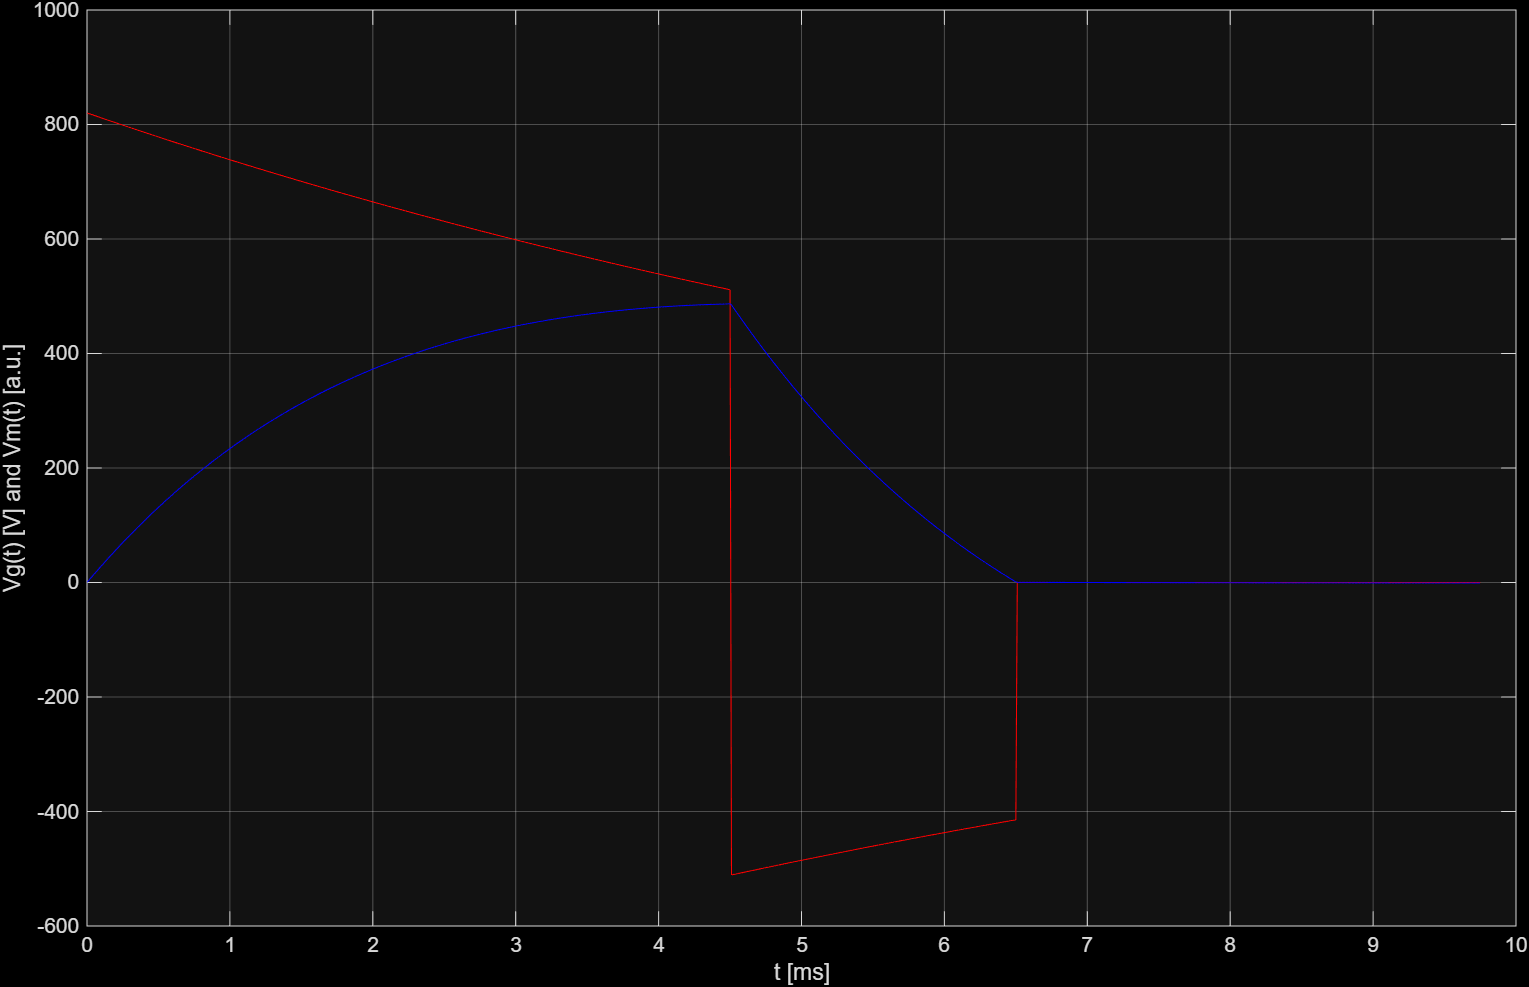
\includegraphics[width=0.7\textwidth]{phase2_response.png}
	\caption{\textcolor{red}{\textbf{Stimulus}} \& \textcolor{blue}{\textbf{Membrane}} Voltage Response over Time, Optimized for $t_{d2}$}
	\label{fig:phase2}
\end{figure}


\section*{Question 2c}
\addcontentsline{toc}{section}{Question 2c}  % add to ToC

Choose one of the values of $\tau_m$ obtained in part (b) to assume when tuning durations. Provide 

The two  reasons for choosing $\tau_m$ optimized for $t_{d2}$ are below.


The plot of the membrane response for tau-m optimized for the  first phase leaves a higher residual voltage after the second phase. This is bad for two reasons.

\begin{enumerate}
	\item It means energy was wasted to get the membrane voltage lower than 0, during the repolarization phase of the stimulus, which will shorten battery life for 0 reasonable gain.
	
	\item Physiologically, the residual voltage across a membrane will make it more difficult for the next depolarization phase, this is because more time will be required to reach resting potential
\end{enumerate}


\section*{Question 3a}
\addcontentsline{toc}{section}{Question 3a}  % add to ToC

Compare the appropriateness of the article’s fixed-tilt and tuned-duration waveforms for patients 
whose actual $\tau_m$ differs from the assumed  $\tau_m$ you inferred in Question 2 for the DeFT Response 
algorithm. For each patient, a complete response will state which of the two waveforms provides 
a more preferable $V_m(t)$ response, support that decision with quantitative observations from 
\texttt{ biphasic\_exp\_fixed\_tilt.m } and \texttt{ biphasic\_exp\_tuned\_dur.m }, and illustrate those 
observations with relevant graphical output from the two scripts. Compare the response to the fixed-tilt and tuned-duration waveforms for a patient with $\tau_m$ = 2.0 ms, which is commonly assumed to be the minimum realistic value of  $\tau_m$. 

We can use MATLAB to help decide what is better for a patient with  $\tau_m = 2.0$ ms. But first as the question asked we should plot both the \textbf{tuned-duration} and the \textbf{fixed-tilt} waveform for this patient. These waveforms can be seen in Figure \ref{fig:3} and Figure \ref{fig:4} respectively.

\begin{figure}[H]
	\centering
	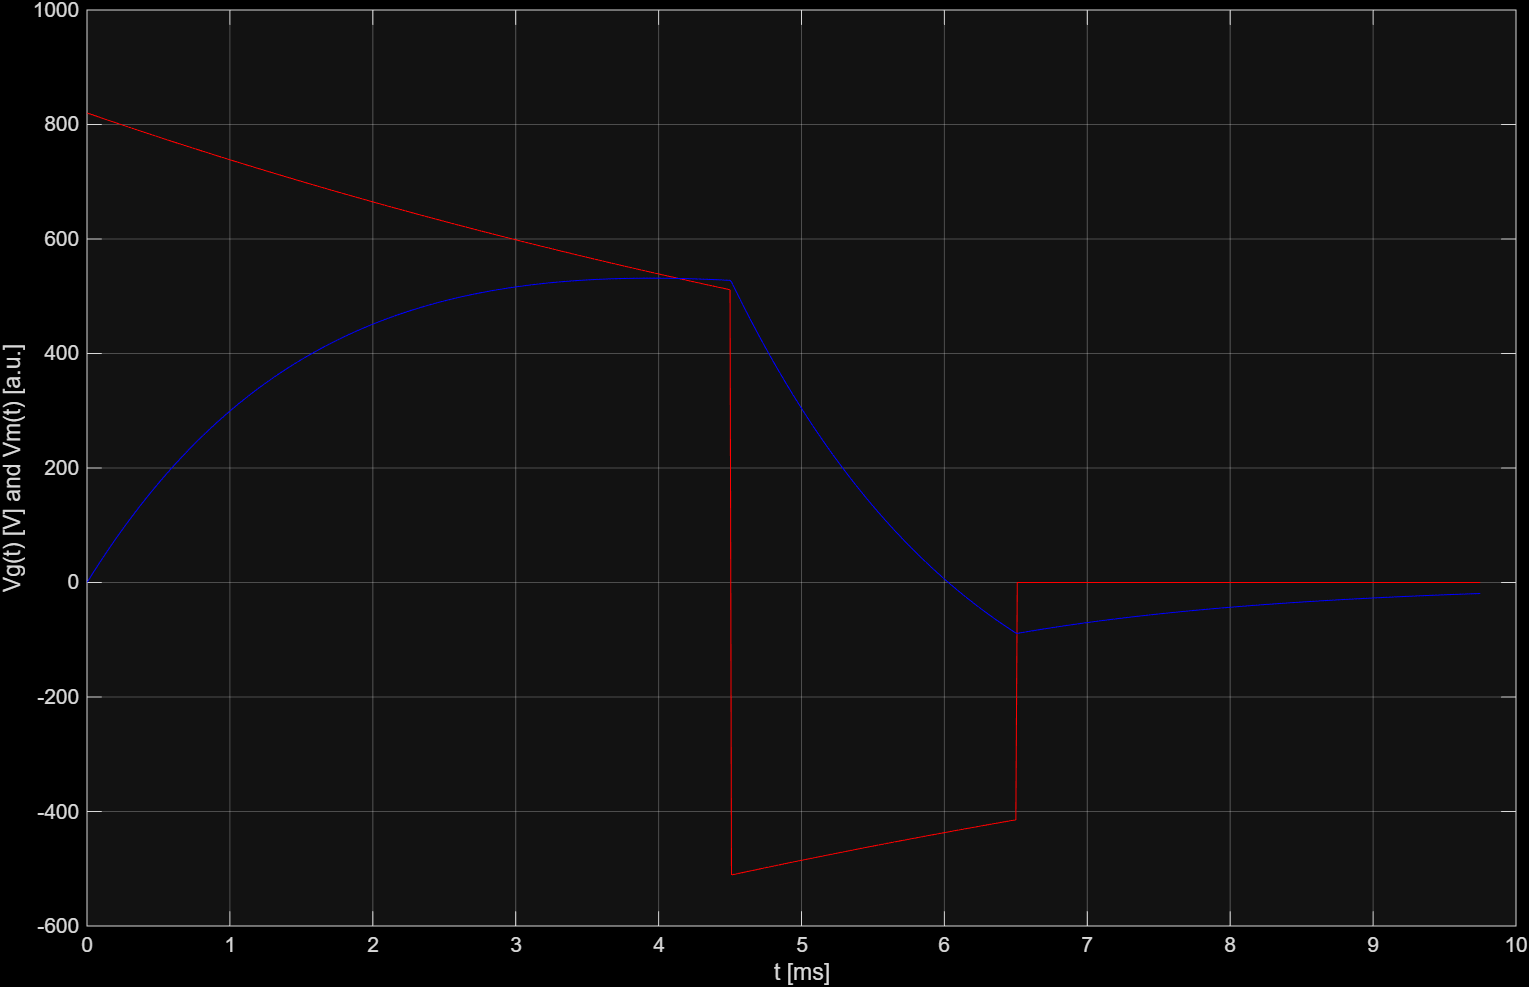
\includegraphics[width=0.7\textwidth]{tau2ms_tuned_dur.png}
	\caption{\centering Tuned-Duration \textcolor{red}{\textbf{Stimulus}} and \textcolor{blue}{\textbf{Membrane}} Voltage Response over Time, with $\tau_m = 2.0$ ms}
	\label{fig:3}
\end{figure}

\begin{figure}[H]
	\centering
	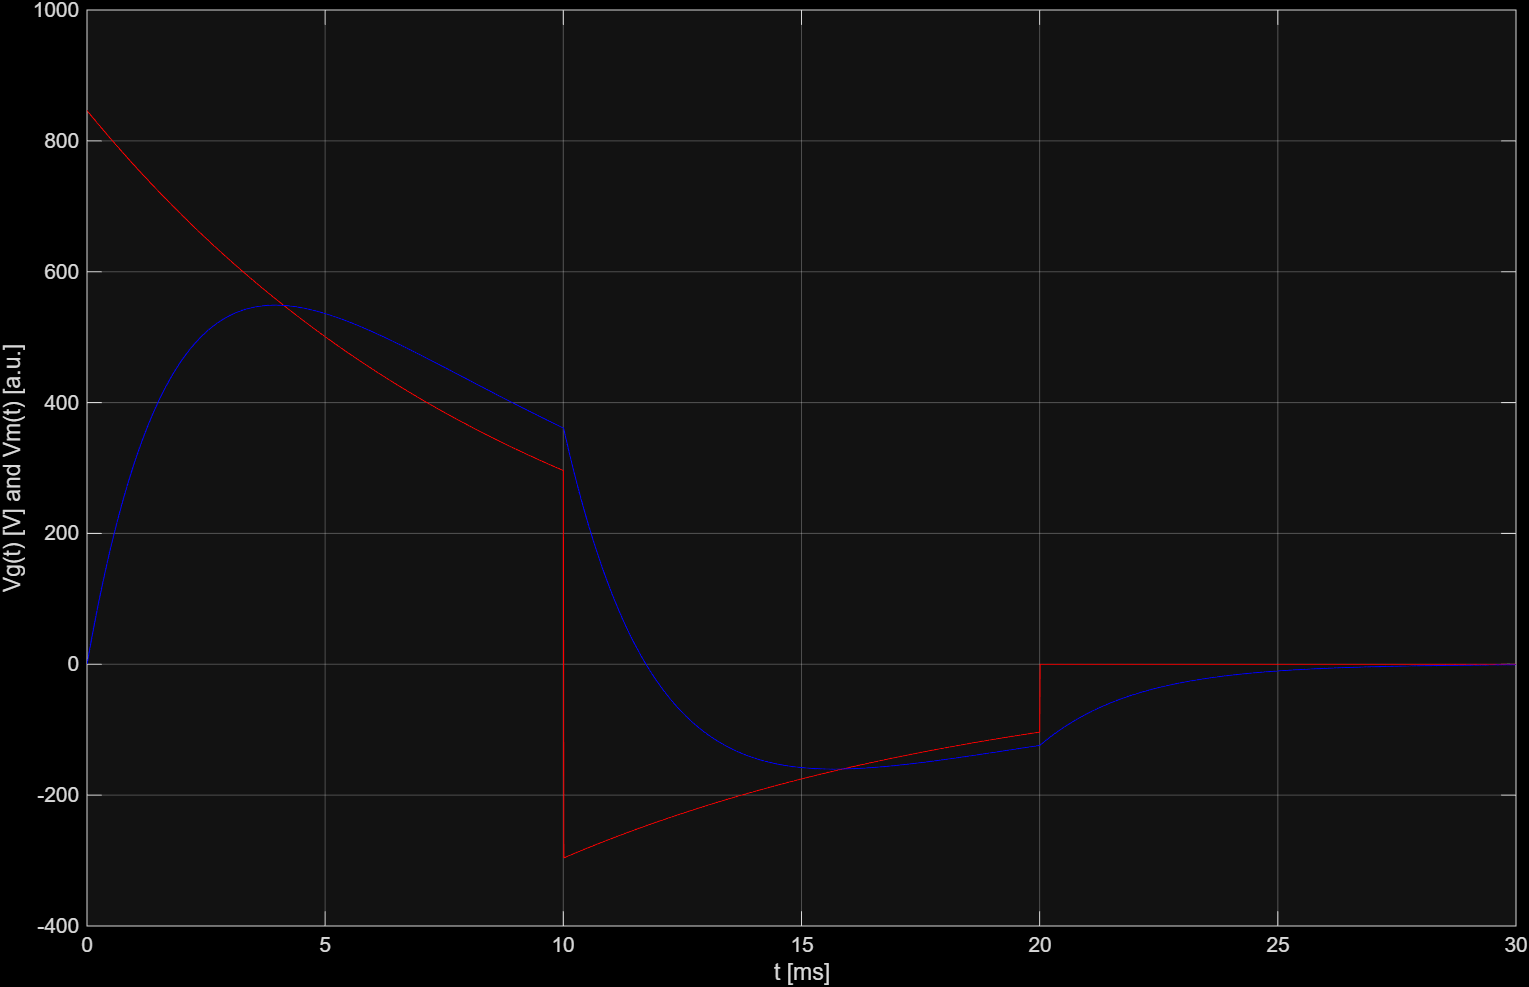
\includegraphics[width=0.7\textwidth]{tau2ms_fixed_tilt.png}
	\caption{\centering Fixed-Tilt \textcolor{red}{\textbf{Stimulus}} and \textcolor{blue}{\textbf{Membrane}} Voltage Response over Time, with $\tau_m = 2.0$ ms}
	\label{fig:4}
\end{figure}

To choose which is preferred we can add a few lines of MATLAB to determine the key characteristics of each waveform. The \textbf{peak voltage} at $t_{d1}$ and the \textbf{residual charge} leftover at $t_{d1} + t_{d2}$.

Both waveforms have different peak voltages, the peaks of each are 531.58 V and 548.93 V for the tuned-duration and fixed-tilt waveforms respectively. If we express both of these values as a percentage of the peak fixed-tilt voltage we can see that the tuned-duration voltage is a $\approx 3$\% lower. 

Both waveforms also have different residual charges left at time, equating to a residual voltage of $t_{d1} + t_{d2}$. -88.26 V and -123.95 V for the tuned-duration and fixed-tilt waveforms respectively. Once again we should express these as a percentage of the peak fixed-tilt voltage so we can have an apples-to-apples comparison of percentages. Doing this shows that the tuned-duration has 16.08 \% and fixed-tilt has a 22.58 \% residual voltage. A table is provided summarizing these values

\begin{table}[H]
	\centering
	\begin{tabular}{@{}lcc@{}}
		\toprule
		$\tau_m$ = 2.0 ms                     & Tuned-Duration Waveform & Fixed-Tilt Waveform \\ \midrule
		Peak Voltage {[}V{]}                  & 531.582               & 548.936             \\
		Residual Voltage {[}V{]}              & -88.263                 & -123.957           \\
		Peak Voltage {[}\% $\text{V}_\text{max}${]}  & 96.84                   & 100                 \\
		Residual Voltage {[}\% $\text{V}_\text{max}${]} & 16.08                   & 22.58              
	\end{tabular}
\end{table}

Overall, I think the tuned-duration waveform is better for this patient with $\tau_m$ = 2.0 ms, as it features ~6.5\% lower residual voltage, with only a ~3\% lower peak voltage.

The MATLAB code that produces these plots and numbers is given below, this will be reused for question 3b, but changing the \texttt{ tau\_m } value to 5.0 ms instead

\begin{lstlisting}[style=Matlab-editor, backgroundcolor=\color{smoky}, basicstyle=\ttfamily\tiny]
clear all;

%% load in previously found C-g tau-g
C_g   = 113.397; % uF
tau_g = 9.5254;  % ms

%% load in tuned duration paper numbers
R_meas    = 84;   % Ohm
t_d1_td   = 4.5;  % ms
t_d2_td   = 2.0;  % ms
E_td      = 28.4; % J

%% load in fixed tilt paper numbers
t_d1_ft   = 10;   % ms
t_d2_ft   = 10;   % ms
tilt_d1   = 0.65; % percent
tilt_d2   = 0.65; % percent
E_ft      = 40;   % J


%% load in 2ms tau-m for 3a)
tau_m = 2.0; % ms

% plot the response for tuned dur
[Vg_td, Vm_td, t_td] = biphasic_exp_tuned_dur(tau_m, C_g, E_td, R_meas, t_d1_td, t_d2_td, 'y');

% plot the response for fixed tilt
[Vg_ft, Vm_ft, t_ft] = biphasic_exp_fixed_tilt(tau_m, C_g, E_ft, R_meas, tilt_d1, tilt_d2, 'y');

%% measure each waveforms peak
peak_td = max(Vm_td);
peak_ft = max(Vm_ft);

%% measure each waveforms residual charge at td2
time_td2_td = (t_d1_td + t_d2_td);
time_td2_ft = (t_d1_ft + t_d2_ft);
fprintf('td2 (TD): %.1f | td2 (FT): %.1f\n', time_td2_td, time_td2_ft);

% get index of each timestamp
idx_td2_td = find( abs(t_td - time_td2_td) == min(abs(t_td - time_td2_td)));
idx_td2_ft = find( abs(t_ft - time_td2_ft) == min(abs(t_ft - time_td2_ft)));

fprintf('idx_td2 (TD): %d | idx_td2 (FT): %d\n', idx_td2_td, idx_td2_ft);

%% print peak volatges, and % deviation
fprintf('Peak (TD): %f | Peak (FT): %f\n', peak_td, peak_ft);
peak_td = peak_td / peak_ft;
peak_ft_n = 1.00;
fprintf('Peak (TD %%max): %.2f | Peak (FT %%max): %.2f\n', 100*peak_td, 100*peak_ft_n);

% get residual
residual_td = Vm_td(idx_td2_td);
residual_ft = Vm_ft(idx_td2_ft);
fprintf('Residual Charge (TD): %f | Residual Charge (FT): %f\n', residual_td, residual_ft);



% find residual as a percentage of the max
residual_td = abs(residual_td) / peak_ft;
residual_ft = abs(residual_ft) / peak_ft;
fprintf('Residual Charge (TD %%max): %.2f | Residual Charge (FT %%max): %.2f\n', 100*residual_td, 100*residual_ft);
\end{lstlisting}


\section*{Question 3b}
\addcontentsline{toc}{section}{Question 3b}  % add to ToC

Here we will repeat the analysis from 3a but with $\tau_m = 5.0$ ms. Since the reasoning was explained previously in 3a it will not be rewritten here. The script used for 3b is also the same as the script from 3a, although with the \texttt{ tau\_m } variable having its value changed to 5.0

The plots for this patient can be found in Figures \ref{fig:5} and \ref{fig:6}

\begin{figure}[H]
	\centering
	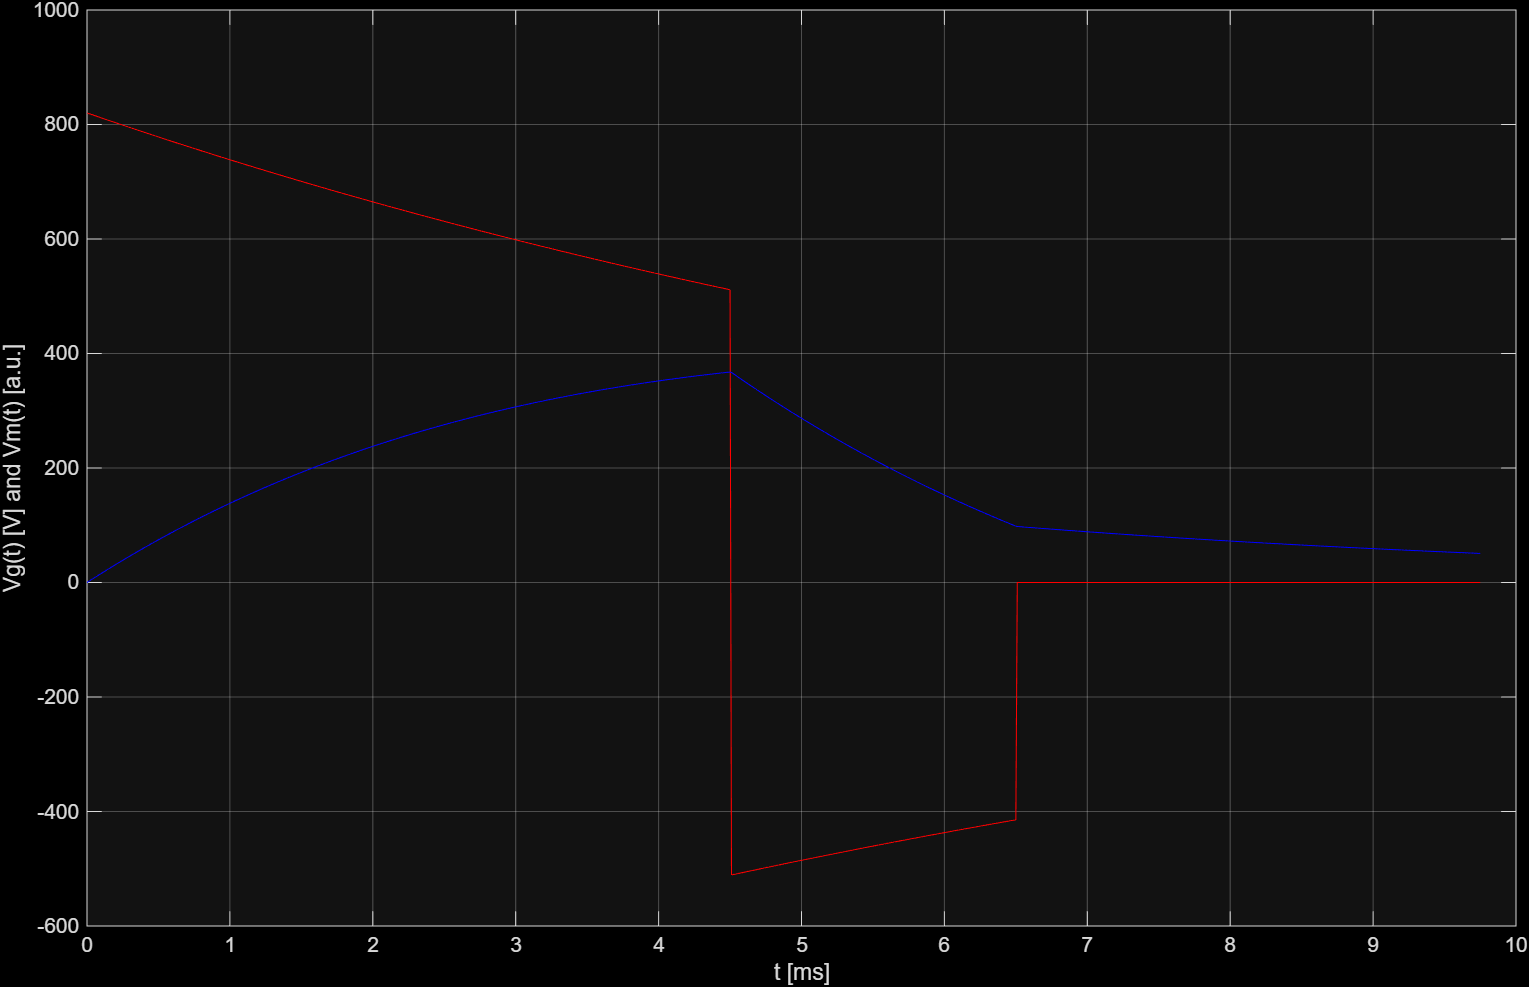
\includegraphics[width=0.7\textwidth]{tau5ms_tuned_dur.png}
	\caption{\centering Tuned-Duration \textcolor{red}{\textbf{Stimulus}} and \textcolor{blue}{\textbf{Membrane}} Voltage Response over Time, with $\tau_m = 2.0$ ms}
	\label{fig:5}
\end{figure}

\begin{figure}[H]
	\centering
	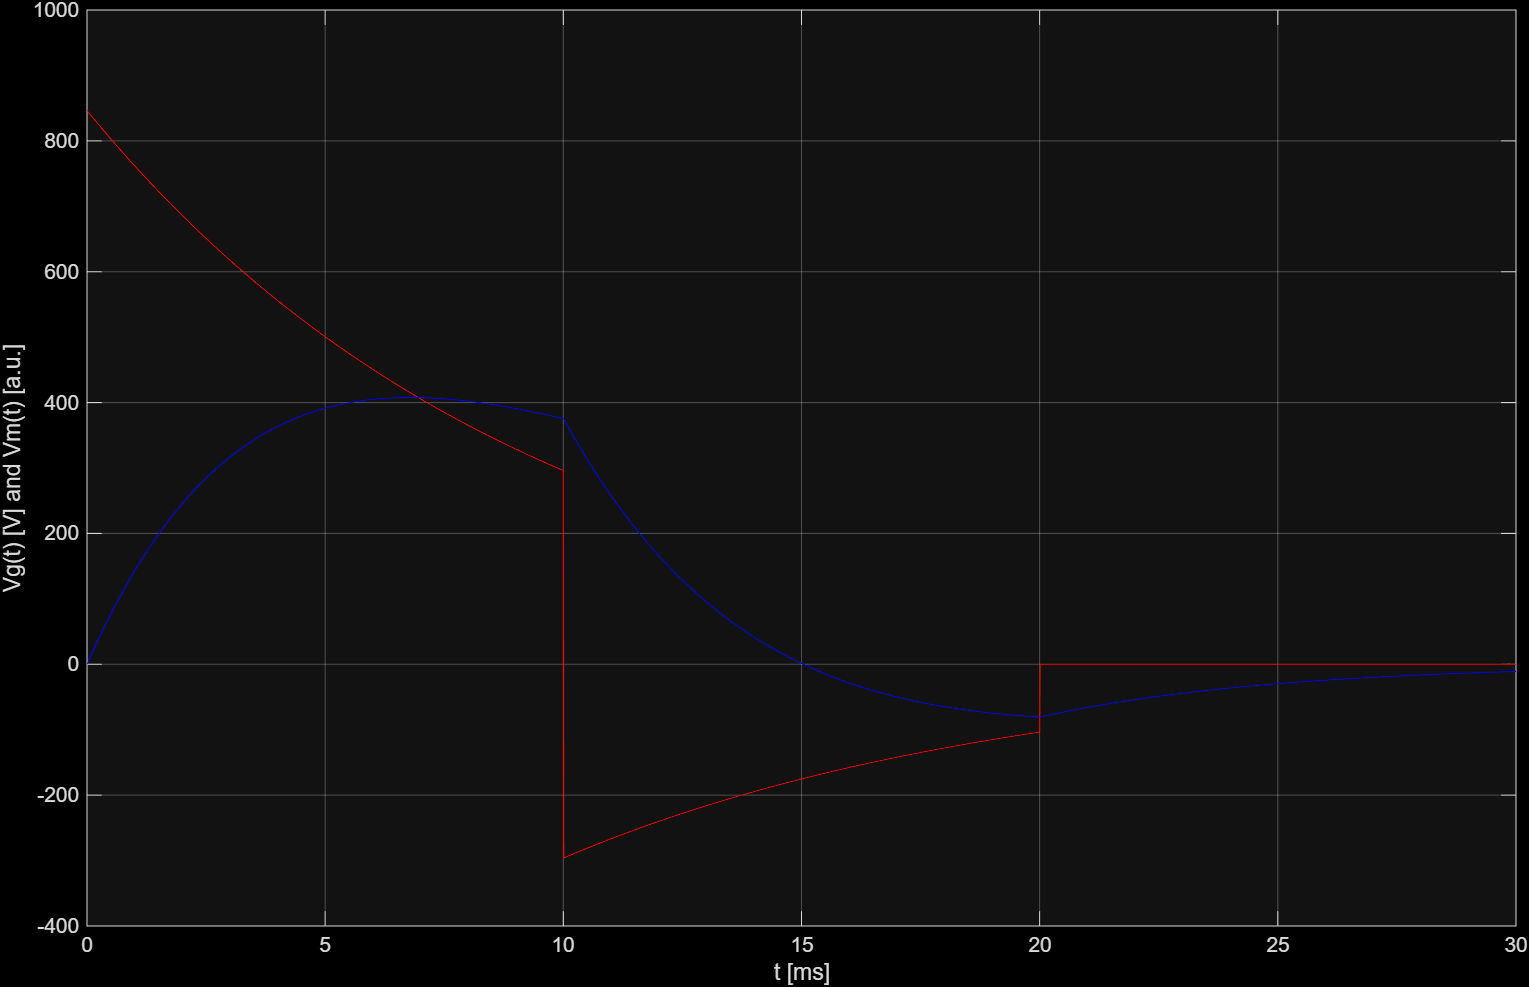
\includegraphics[width=0.7\textwidth]{tau5ms_fixed_tilt.png}
	\caption{\centering Fixed-Tilt \textcolor{red}{\textbf{Stimulus}} and \textcolor{blue}{\textbf{Membrane}} Voltage Response over Time, with $\tau_m = 2.0$ ms}
	\label{fig:6}
\end{figure}

The statistics I previously discussed are put in the below table for comparison, note that the residual voltage percentage is now signed to distinguish between positive residual voltage, and negative residual voltage

\begin{table}[H]
	\centering
	\begin{tabular}{@{}lcc@{}}
		\toprule
		$\tau_m$ = 5.0 ms                     & Tuned-Duration Waveform & Fixed-Tilt Waveform \\ \midrule
		Peak Voltage {[}V{]}                  & 367.635                 & 407.738             \\
		Residual Voltage {[}V{]}              & 98.441                  & -80.507             \\
		Peak Voltage {[}\% $\text{V}_\text{max}${]}  & 90.16                   & 100                 \\
		Residual Voltage {[}\% $\text{V}_\text{max}${]} & 24.14                   & -19.74              
	\end{tabular}
\end{table}

For this patient the fixed-tilt waveform is preferable due to the higher peak voltage and the lower residual voltage the waveform possesses. Another reason we prefer the fixed-tilt is due to the fact that the tuned duration fails to repolarize the membrane


\section*{Question 4a}
\addcontentsline{toc}{section}{Question 4a}  % add to ToC

Is there anything special about specifying duration rather than tilt? Explore this question by 
completing the following steps. Compute $V_m(t)$ for the article’s tuned-duration waveform assuming the patient’s actual $\tau_m$ is equal to the assumed $\tau_m$ you obtained in Question 2. For full marks, specify the command line you used to call \texttt{ biphasic\_exp\_tuned\_dur.m } and plot the Vm(t) result you obtained. 

This is a one-liner of MATLAB code that we can type in the command window

\begin{lstlisting}[style=Matlab-editor, backgroundcolor=\color{smoky}]
>>  biphasic_exp_tuned_dur(2.7270, 113.397, 28.4, 84, 4.5, 2.0, 'y');
\end{lstlisting}

The plot for this is shown in Figure \ref{fig:7}

\begin{figure}[H]
	\centering
	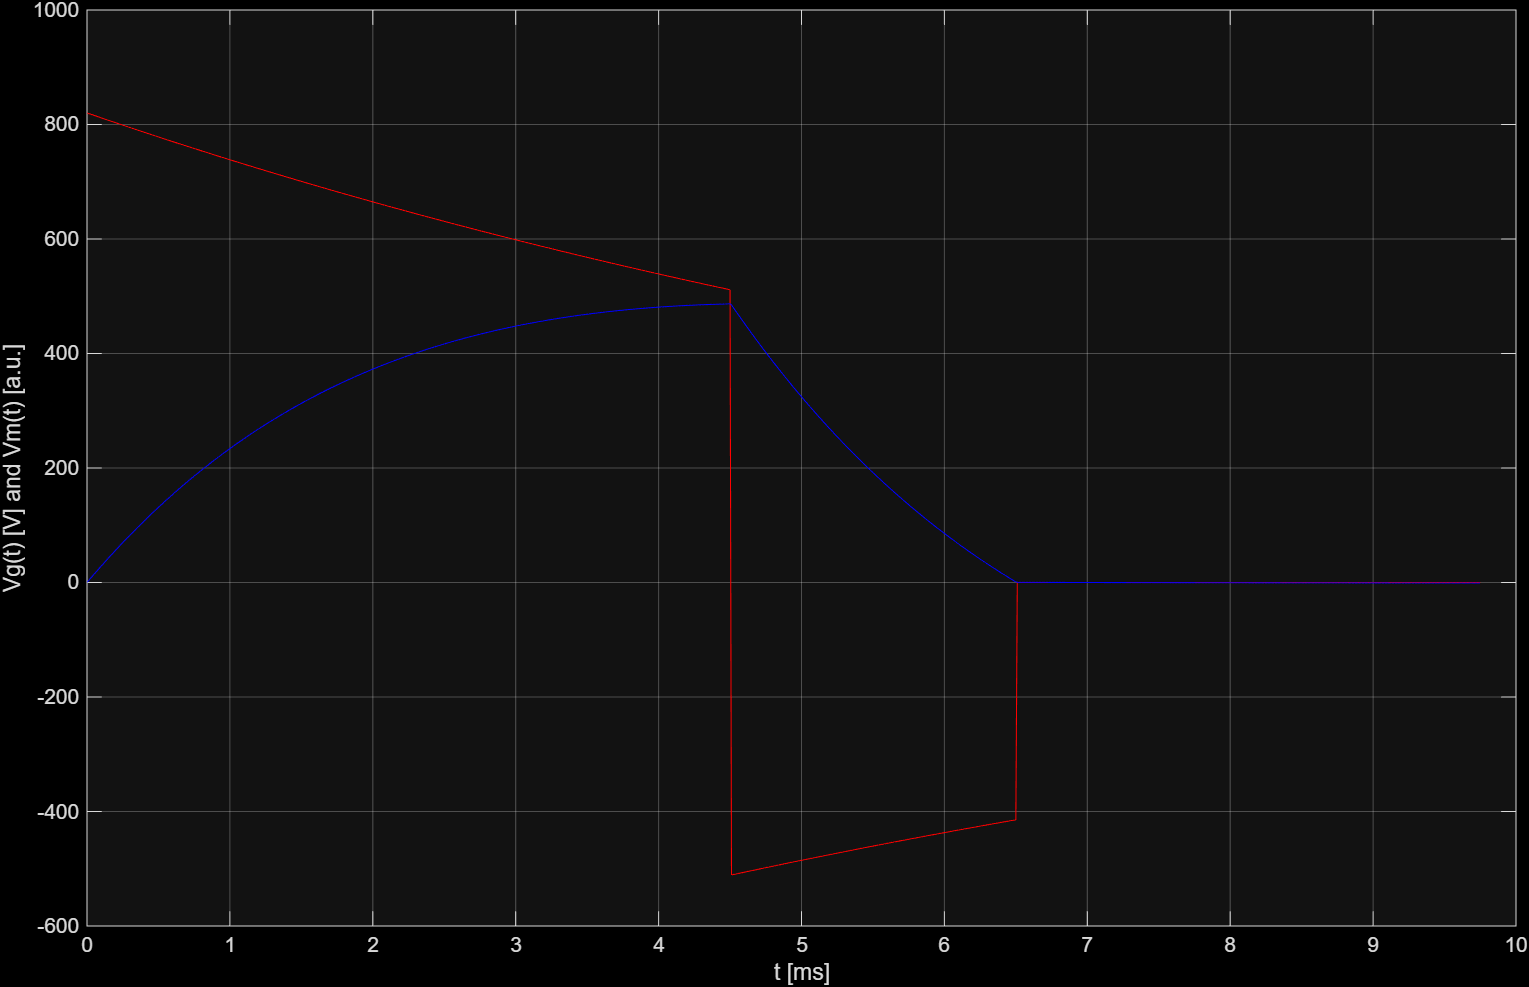
\includegraphics[width=0.7\textwidth]{q4_response.png}
	\caption{\centering Tuned-Duration \textcolor{red}{\textbf{Stimulus}} and \textcolor{blue}{\textbf{Membrane}} Voltage Response over Time, with $\tau_m = 2.7270$ ms}
	\label{fig:7}
\end{figure}

\section*{Question 4b}
\addcontentsline{toc}{section}{Question 4b}  % add to ToC

To design a fixed-tilt waveform that is equivalent to our tuned-duration waveform we start by analyzing the system. Here we have a linear, time-invariant (LTI) model for the myocardium. This means that the input $X(s)$ maps to some output $Y(s)$ through a transfer function $H(s)$. This is shown in equation \ref{eq:5}

\begin{equation}
\label{eq:5}
Y(s) = H(s) \cdot X(s)
\end{equation}

In other words, the same input waveform will always produce the same output waveform. This means to find a fixed-tilt waveform with the same output response as our tuned-duration waveform, we need to ensure that the input waveform (stimulus) is the same.

A fixed-tilt waveform's \textit{shape} is defined by 2 parameters, the tilts of phase 1 and 2. Since the fixed-tilt waveform also follows exponential decay, it also follows capactive discharge, and we should be able to completely equate both waveforms.

To do this lets look at equation \ref{eq:1} Which relates duration and tilt through capacitive discharge. We can use our phase durations from the tuned-duration waveform here to calculate the required tilts.

\textit{Note:} At this stage in the assignment the value of $\tau_g$ is known.

\[
	\text{Tilt}_{d1} = 1 - \exp{\left( - \frac{t_{d1}}{\tau_g} \right)} = 1 - \exp{\left( - \frac{4.5 \text{m}}{9.5254 \text{m}} \right)} = 0.3765
\]

\[
	\text{Tilt}_{d2} = 1 - \exp{\left( - \frac{t_{d2}}{\tau_g} \right)} = 1 - \exp{\left( - \frac{2.0 \text{m}}{9.5254 \text{m}} \right)} = 0.1893
\]

This gives phase 1 and 2 tilts of 37.65\% and 18.93\% respectively. These values determine the \textit{shape} of the waveform, but for the \textit{amplitude} of the fixed-tilt waveform to match the tuned-duration we must ensure we deliver the same energy. This means reusing the $E$ value of 28.4J from the tuned-duration waveform. The other parameters $C_g$ and $\tau_m$  determine the patients response, so these will be fixed between both waveforms, $R_\text{meas}$ is partially determined by the hardware as well, since the same hardware is used for both waveforms this value will also be fixed.

With this analysis we can say that tuned-duration and fixed-tilt waveforms are essentially two ways to represent the same thing. This statement holds as long as the same hardware is used to generate both waveforms, which in our case is true as the mechanism is capacitive discharge in both cases.

In general if we define TD() as a function determining a tuned-duration waveform stimulus in equation \ref{eq:td}, and FT() as a function determining a fixed-tilt waveform stimulus in equation \ref{eq:ft}. 

\begin{equation}
\label{eq:td}
\text{TD}\left( t_{d1}, \, t_{d2}, \, E \right)
\end{equation}

\begin{equation}
\label{eq:ft}
\text{FT}\left( \text{tilt}_{d1}, \, \text{tilt}_{d2}, \, E \right)
\end{equation}

We can say the following holds true.

\[
\text{TD}\bigg( t_{d1}, \,\, t_{d2}, \,\, E \bigg) = \text{FT}\left( 1 - \exp{\left[ - \frac{t_{d1}}{\tau_g} \right]}, \,\, 1 - \exp{\left[ - \frac{t_{d2}}{\tau_g} \right]}, \,\, E \right)
\]

To plot this newly designed fixed tilt waveform in MATLAB we can use the following line:

\begin{lstlisting}[style=Matlab-editor, backgroundcolor=\color{smoky}]
>>  biphasic_exp_fixed_tilt(2.7270, 113.397, 30, 84, 0.3765, 0.1893, 'y');
\end{lstlisting}

Figure \ref{fig:8} shows the response of this newly-designed fixed tilt stimulus. Figure \ref{fig:9} shows both the Tuned-Duration and Fixed-Tilt response waveforms on the same axes

\begin{figure}[H]
	\centering
	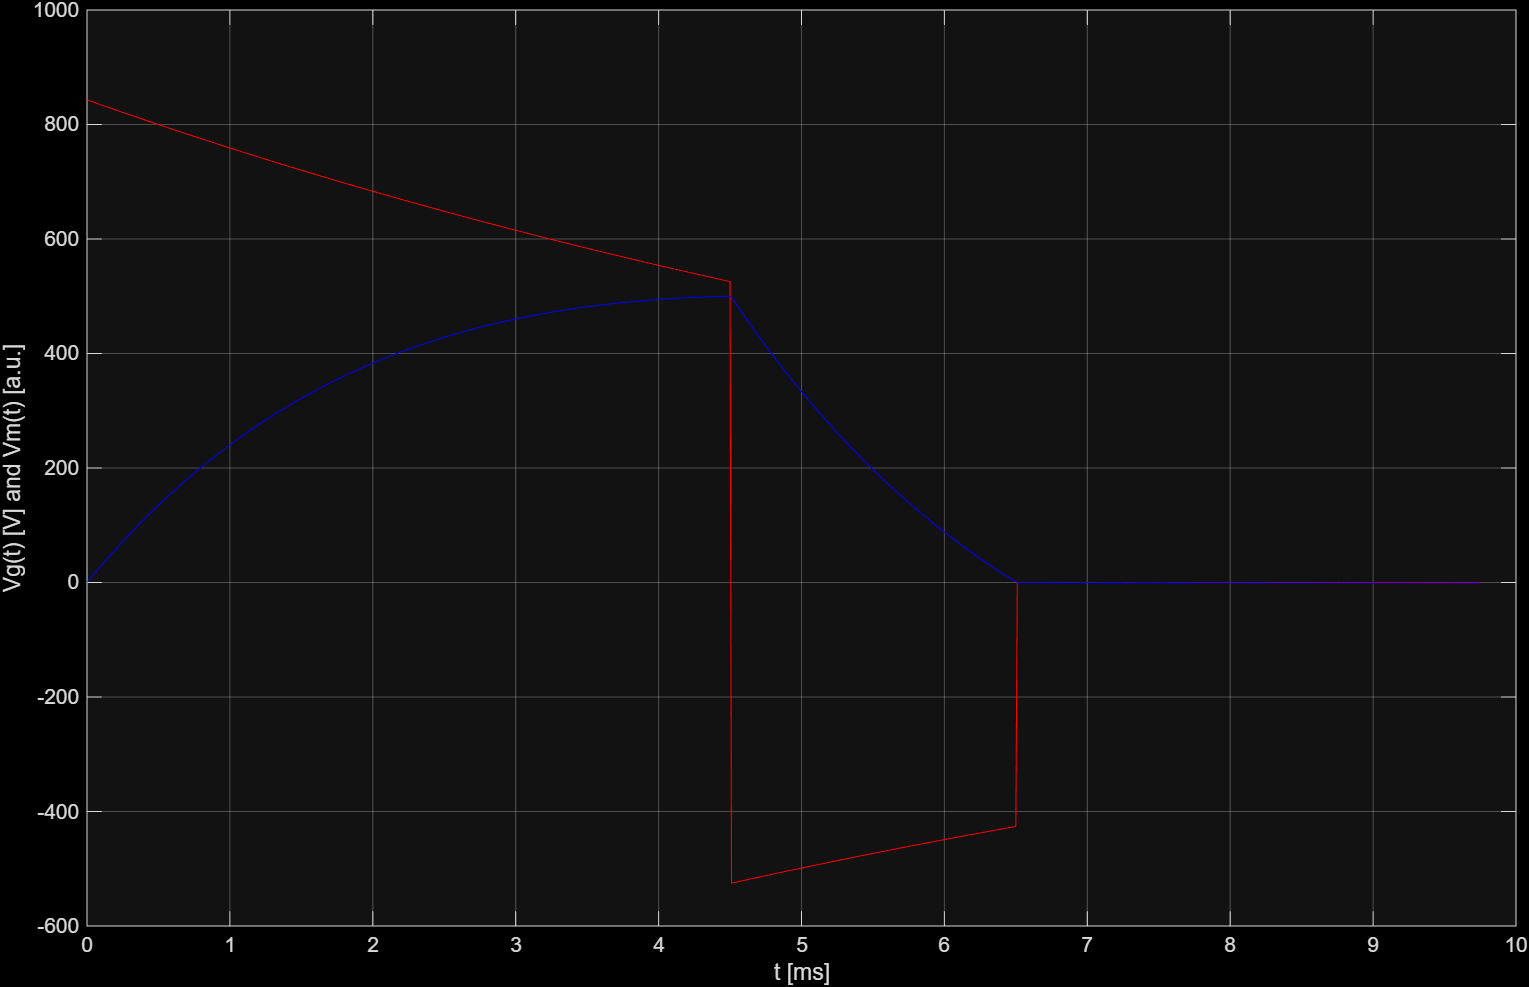
\includegraphics[width=0.7\textwidth]{q4_response2.png}
	\caption{\centering New Fixed-Tilt \textcolor{red}{\textbf{Stimulus}} and \textcolor{blue}{\textbf{Membrane}} Voltage Response over Time, with $\tau_m = 2.7270$ ms}
	\label{fig:8}
\end{figure}

\begin{figure}[H]
	\centering
	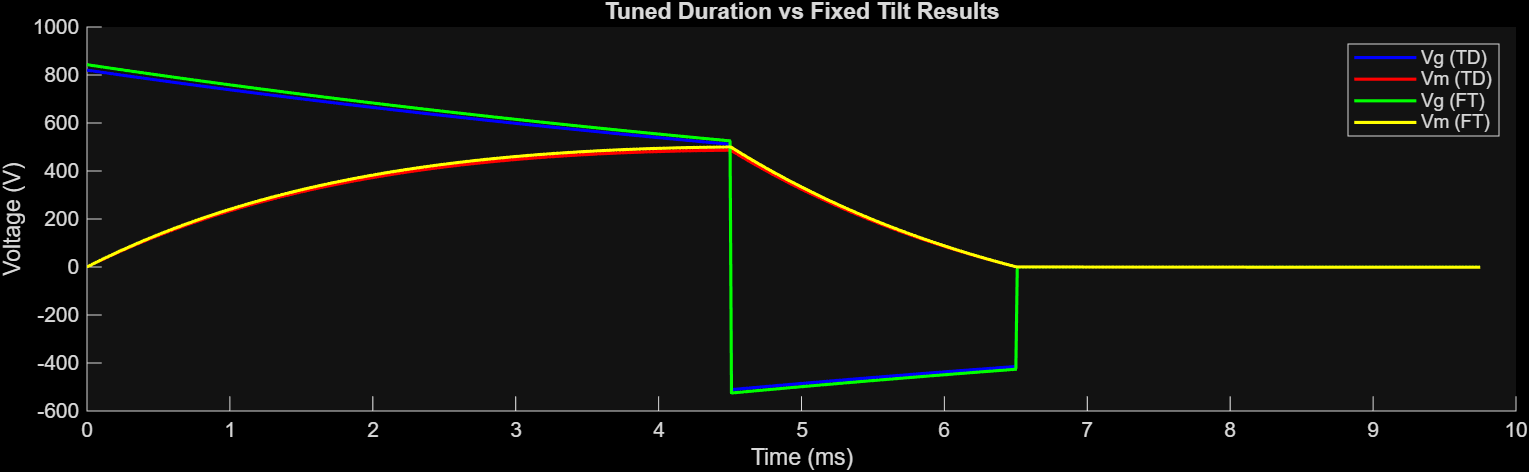
\includegraphics[width=0.9\textwidth]{td_vs_ft.png}
	\caption{\centering New Fixed-Tilt and Tuned-Duration Voltage Response over Time, with $\tau_m = 2.7270$ ms}
	\label{fig:9}
\end{figure}

The MATLAB script used to plot Figures \ref{fig:7} - \ref{fig:9} is given below:

\begin{lstlisting}[style=Matlab-editor, backgroundcolor=\color{smoky},  basicstyle=\ttfamily\tiny]
%% load in previously found C-g tau-g
C_g   = 113.397; % uF
tau_g = 9.5254;  % ms

%% load in tuned duration paper numbers
R_meas    = 84;   % Ohm
t_d1_td   = 4.5;  % ms
t_d2_td   = 2.0;  % ms
E_td      = 28.4; % J

tau_m = 2.7270; % ms

[Vg_td, Vm_td, t_td] = biphasic_exp_tuned_dur(2.7270, 113.397, 28.4, 84, 4.5, 2.0, 'y');

%% q 4b

[Vg_ft, Vm_ft, t_ft] = biphasic_exp_fixed_tilt(2.7270, 113.397, 30, 84, 0.3765, 0.1893, 'y');

% analyze the results from the tuned duration and fixed tilt experiments
figure;
subplot(2,1,1);       % first subplot
hold on;               % keep all plots on the same axes

% plot everythign
plot(t_td, Vg_td, 'b', 'LineWidth', 1.5);
plot(t_td, Vm_td, 'r', 'LineWidth', 1.5);
plot(t_ft, Vg_ft, 'g', 'LineWidth', 1.5);
plot(t_ft, Vm_ft, 'y', 'LineWidth', 1.5);

% lables
xlabel('Time (ms)');
ylabel('Voltage (V)');
title('Tuned Duration vs Fixed Tilt Results');
legend('Vg (TD)', 'Vm (TD)', 'Vg (FT)', 'Vm (FT)');

hold off;
\end{lstlisting}

\end{document}